% Konzept

\chapter{Konzept}
\label{konzept}

Im folgenden werden Konzepte diskutiert, um die in Kapitel \ref{anforderung} herausgearbeiteten Anforderungen zu erfüllen.

\section{Implementierungsziele}
Ziel des Arbeit ist es eine prototypische AR- bzw. VR-Anwendung zur Visualisierung und Untersuchung von MRT-Daten zu implementieren. 

Vor allem was den Bereich der Volumendarstellung angeht, gibt es bereits viele Programme und Arbeiten, die diese erfolgreich umsetzten, wie im Kapitel \ref{grundlagen} erläutert wurde.
Wie später beschrieben, wurden diese teilweise als Grundlage für die Anwendung verwendet. Die Anwendung soll mit der Spiele Engine Unity 3D implementiert werden, worauf ebenfalls im späteren Kapiteln eingegangen wird. Die Lösung muss also damit kompatibel sein. In Kapitel \ref{grundlagen} wurde unter anderem die Unity-Erweiterung Volume Viewer Pro beschrieben, die viele der gestellten Anforderungen bereits abdeckt. Das Programm ist allerdings kostenpflichtig. Eine unabhängige und frei zugängliche Software ist dem allerdings vorzuziehen, vor allem, da es sich um einen Prototyp handelt, der Aufschluss über die Verwendungsmöglichkeiten in diesem Bereich liefern und daher eventuell weiterentwickelt werden soll. Deshalb sollte die dreidimensionale Darstellung im Rahmen dieser Arbeit entwickelt werden und Code aus anderem Quellen nur verwendet werden, wenn er diesen Kriterien entspricht.

\section{3D Darstellung}

Im Kapitel\ref{grundlagen} wurden verschiedene Methoden vorgestellt, um ein Volumen zu visualisieren. An dieser Stelle soll diskutiert werden, welche davon sich am besten für die Umsetzung in mARt eignet.
Die 3D-Darstellung sollte die in Kapitel \ref{anforderung} beschriebenen Eigenschaften haben:

\begin{itemize}
\item Darstellung sollte das Volumen dreidimensional abbilden. \textbf{(U03)}
\item Die innere Struktur des Gehirns sollte erkennbar sein \textbf{(U01)}
\item Die Markierung des vom Schlaganfall betroffenes Bereichs sollte die MRT-Darstellung nicht unkenntlich machen. \textbf{(U12)}
\item Es sollte möglich sein durch die Schichten des Volumes zu scrollen. \textbf{(U07)}
\end{itemize}

Dadurch lassen sich Aussagen über das Aussehen der Darstellung herleiten.
Da das innere der 3D Darstellung erkennbar sein soll, muss eine semi-transparente Darstellung erzeugt werden, die sowohl die Form des Gehirns abbildet, als auch die innere Struktur. Die eingeblendete Markierung sollte ebenfalls zu einen gewissen Grad transparent sein.
Weiterhin sind sind nur die Pixel relevant, die das Gehirn darstellen. Der Bereich darum (Schädel und Hintergrund) sollten gefiltert  und nicht sichtbar gemacht werden. Das gewünschte Ergebnis ist, dass das Gehirn frei im Raum "schwebt". 

Die Anforderungen sprechen gegen eine Umsetzung, die eine Oberfläche des Gehirns erzeugt und es als Mesh darstellt. Die Form des Gehirns könnte dadurch deutlich gezeigt werden und das Objekt würde von den umgebenden Pixeln getrennt werden. 
Allerdings handelt es sich bei dem Gehirn nicht um eine Hülle sondern eher eine Masse. Es ist unwahrscheinlich, dass ein Verfahren wie Marching Cubes die inneren Gehirnstrukturen exakt genug wiedergeben könnte, damit ein Neurologe sinnvolle Schlüsse daraus ziehen kann. Weiterhin müsste das Mesh in Echtzeit kontinuierlich angepasst werden, wenn der Nutzer durch die verschiedenen Schichten scrollt. 
Deshalb eignet sich eine Oberflächengenerieurung nicht zur Visualisierung.
Hinzu kommt, dass in den Anforderungen kein Anwendungsfall beschrieben wird, der eine Oberfläche erfordert. Dies würde z.B. gelten, wenn 	
	- Im Fokus der Darstellung, soll das Innere des Gehirns stehen. Ein Mesh, dass die äußere Form beschreibt ist also nicht sinnvoll, zumal keine der Anforderungen Funktionen beschreibt, für die ein Mesh nötig wäre (z.B. Kollsion (Unity)
	
Die dreidimensionale Darstellung lässt sich also besser mit einer Volume Rendering Methode umsetzten. 
Aus den in Kapitel \ref{grundlagen} beschriebenen Methoden wurde das Volume Ray Casting ausgewählt. 
WARUM?

Wie in dem Kapitel \ref{grundlagen} beschrieben, gibt es bereits viele Lösungsansätze zur 3D Darstellung von MRT-Bildern. Obwohl verschiedene Methodne zum Einsatz kommen, ist der am weitesten verbreitete Ansatz der des Volume Rendering.
Dies hat die folgenden Gründe:
- 
- ...
	
Diese Vorgehensweise ist somit am besten für die Implementierung der Anwendung geeignet.
Diese wird im Kapitel \ref{implementierung} genauer beschrieben.

Anforderungen an Shader??

In Kapitel \ref{grundlagen} wurden die verschiedenen Volume Render Techniken mit einander verglichen. D

%//TODO:
Argumentation für verwendete Technik

Wie im Kapitel \ref{grundlagen} beschrieben, werden beim Volume Rendering in der Regel Transferfunktionen eingesetzt, um verschiedene Gewebestrukturen oder Materialien zu unterscheiden. Wobei es sich um eine Look-Up-Tabelle in Form einer Textur handelt, die jedem Isowert eine Farbe und Opazität zuweist.
Die Herausforderung bei der Implementierung einer Transferfunktion ist dabei die Generierung einer zum Datensatz passenden Textur. Selbst bei einer Transferfunktion mit nur einer Dimension müssen häufig verschiedene Wertzuweisungen ausprobiert werden, um ein gutes Ergebnis zu erhalten.
Um eine bzw. mehrere Transferfunktionen zu genieren, die den Ansprüchen des Nutzers genügt und die für verschiedene Datensätze passend sind, ist es deshalb sinnvoll dem Nutzer eine Benutzeroberfläche zur Verfügung zu stellen, mit deren Hilfe er die verwendete Transferfunktion zur Laufzeit manipulieren kann. 

In einem Volumen gibt es in der Regel bestimmte Isowerte, die Grenzwerte zwischen verschiedenen Materialien darstellen. Diese dienen als Kontrollpunkte, zwischen denen dann interpoliert wird, um einen Farbverlauf zwischen den Materialien zu erhalten. 
Um die Transfertextur zu beeinflussen muss der Nutzer diese Kontrollpunkte verändern können. Zur Umsetzung einer solchen Manipulation eignet sich eine Spline-Interpolation. 
TODO:
Wie funktioniert das?
Die nutzergesteuerte Generierung von Transferfunktionen konnte aus zeitlichen Gründen im Rahmen dieser Arbeit nicht umgesetzt werden.

% ZU MOTIVATION
Weiterhin könnte man anhand des Modells auch Voraussagen von Therapieerfolgen anschaulich demonstrieren.
%%

\section{Darstellung des gekennzeichneten Bereichs}
\label{maske}


In User Story \textbf{U11} der Anforderungen wird beschrieben, dass der vorher von einem Arzt gekennzeichnete Bereich des Gehirn, der vom Schlaganfall betroffen ist in der Darstellung angezeigt werden soll, wenn dies gewünscht ist. 
Der Bereich wird durch Masken definiert, die zuvor von einem Arzt in einem externen Programm erstellt wurden und ebenfalls im NIfTI-Format vorliegen. Für jede Schicht in einem Datensatz existiert ebenfalls eine Schicht im Maskendatensatz. 

Der Bereich soll sowohl in der zwei- als auch in der dreidimensionalen Ansicht dargestellt werden. Bei letzterer sollte er auch in den Querschnitten erkennbar sein, die sich durch das Scrollen durch das Volumen ergeben. Das Verhalten von MRT-Daten und markiertem Bereich ist also gleich.

Da die Daten im selben Format vorliegen und sich gleich verhalten sollen, ist es naheliegend, dass sie auf die selbe Weise implementiert werden. Dementsprechend werden auch die Maskenbilder in eine 3D-Textur übertragen, die dann durch Volume Ray Tracing gerendert wird. Damit aber nicht jeder Strahl doppelt verschossen werden muss, der das Volumen durchdringt, wird der Zugriff auf die Maskentextur in den Shader integriert, der bereits das MRT-Volumen rendert. Für jeden Voxel, der aus der 3D-Textur der MRT-Daten gelesen wird wird  der Voxel mit denselben Koordinaten aus der Masken-3D-Textur gelesen. Die zwei Farbwerte werden zum Schluss miteinander verrechnet. Durch die Verrechnung, bleibt trotzdem die Struktur des Gehirns erkennbar, wie es von \textbf{U12} gefordert wird. Die Abfrage der Maskenwerte erfolgt nur, wenn durch das Material eine entsprechende Steuervariable gesetzt wurde.
Dies wird im folgenden Codebeispiel veranschaulicht.

\begin{minted}[mathescape,
               linenos,
               numbersep=5pt,
               gobble=2,
               frame=lines,
               framesep=2mm]{csharp}
void main(sampler3D _Volume,
		  sampler3D _MaskVolume,
          sampler1D _TransferTexture,
          float3 texCoord : TEXCOORD0,
          float4 maskColor : COLOR,
          float _ShowMask)
{
  // Der Isowert des Volumens wird für die aktuelle Position ausgelesen
  float isoValue = tex3D(_Volume, texCoord);
  
  if (_ShowMask == 1)
  {
		// Der Isowert des Maskenvolumens wird für die aktuelle Position ausgelesen
		float isoValueMask = tex3D(_MaskVolume, texCoord);
  }
	
  // Die Werte werden verrechnet und die Maske wird zusätzlich eingefärbt
  return isoValue * isoValueMask * maskColor;
}
\end{minted}

\section{2D Darstellung}
\textbf{U02}
\section{Endgerät}

Im Kapitel \ref{grundlagen} wurde die Vor- und Nachteile von AR und VR gegenüber gestellt.
Wie bereits im Kapitel \ref{motivation} beschrieben, ist mARt als AR-Anwendung konzipiert. Obwohl die Technologie noch viele Unzulänglichkeiten aufweist, eignet sie sich auf lange Sicht dennoch besser für den Einsatz in einem medizinischen Arbeitsumfeld.
Für den Arbeitsalltag eines Arztes und die Zusammenarbeit mit Patienten eignet sich ein durchsichtiges Display deutlich besser als ein undurchsichtiges. Der Nutzer verliert somit nicht seine Umwelt aus den Augen, wodurch er sich sicherer in der Benutzung fühlt. In einem Anwendungsszenario, in dem er mit anderen Menschen kommuniziert, während er die Anwendung bedient gilt dies umso mehr. Die mögliche Verwendung von mARt während einer Operation oder Behandlung wäre mit einer VR-Anwendung unmöglich. Die Reduzierung auf die virtuelle Realität bietet zudem keinen Vorteil für die Funktion der Anwendung, da die Umwelt in der Anwendung nicht verändert werden soll. 

Ein weiterer Vorteil eines AR-HMDs ist seine Portabilität. Dies ist vor allem entscheidend, wenn die Daten anderen Personen, wie z.B. Patienten gezeigt werden sollen. Das Gerät lässt sich einfach in ein anderes Zimmer mitnehmen, was mit einem VR-System deutlich schwieriger umzusetzen ist.
 
Eine große Einschränkung bietet die geringe Anzahl an Gesten und Interaktionsmöglichkeiten, die bisherige AR Technik zur Verfügung stellen. Dies ist allerdings hinfällig, wenn stattdessen die Leap Motion verwendet wird um Nutzereingaben zu erfassen. Die Vorteile des Gerätes werden im folgenden Abschnitt erläutert.

Es ist zu erwarten, dass sich AR-HMDs in den folgenden Jahren deutlich verbessern werden, was Tragekomfort und Leistungfähigkeit angeht. Da mARt als Prototyp einer medizinischen Anwendung anzusehen ist, kann davon ausgegangen werden, dass bei einer Weiterentwicklung der Anwendung Technologie zur Verfügung steht, die viele der genannten Mängel behebt.

Obwohl sich eine AR-Anwendung also besser für die Umsetzung eignet, ist die Leistung des Gerätes nicht ausreichend, um die intensiven Berechnungen durchzuführen, die für das Volume Ray Casting erforderlich sind. Auch der Einsatz der Leap Motion erfordert eine hohe Rechenleistung.
In einer Demo, in der die 3D-Darstellung auf der Hololens getestet wurde, wurde eine Framerate von X erreicht. 
Dies ist nicht ausreichend, um eine angenehme und effektive Arbeitsweise zu ermöglichen. 

Aus diesem Grund wurde die die AR-Anwendung mit eingeschränkter Funktionalität entwickelt. Für die dreidimensionale Darstellung wurden vorgerenderte Bilder eingesetzt, um Testern eine Vorstellung davon zu geben.
Zusätzlich dazu wurde die Anwendung als VR-Erfahrung umgesetzt. Die Funktionalität bleibt dabei die selbe. 
Durch Verwendung der Motion Leap ist selbst die Interaktion mit dem Modell in beiden Anwendungen identisch. 
% Bezug Hololens2?

%Benchmarks!

%//TODO

\section{Interaktion/ UI } 

In diesem Abschnitt wird das Konzept der Interaktion innerhalb der Anwendung beschrieben. Dazu wird zunächst diskutiert, mit welcher Technik die Nutzereingabe erfasst werden soll. Dann wird auf die Gestaltung der Bedienelemente in der Anwendung eingegangen.

\subsection{Nutzereingabe}
%//TODO:
Referenzen?

Wie bereits im vorherigen Abschnitt erwähnt, wird die Leap Motion in Kombination mit dem jeweiligen HMD benutzt, um den Nutzer mit der Anwendung interagieren zu lassen. 
Die Leap Motion trackt die Hände des Nutzers und stellt diese als 3D-Modelle innerhalb der Anwendung dar. Die Bewegungen der Hände werden dabei sehr genau nachempfunden, sodass die Illusion entsteht die simulierten Hände wären die eigenen. 
Das Gerät fördert den intuitiven Umgang mit der Anwendung enorm und ermöglicht damit ein positives Nutzungserlebnis. Weiterhin wird dadurch das erlernen komplexer Gesten oder die Verwendung von Controllern umgangen. Beides sind Hindernisse, die Nutzer, die mit der Technik nicht vertraut sind abschrecken könnten. 
Nachteilig ist, dass das Sichtfeld der Kamera begrenzt ist. Da diese vorne auf dem HMD angebracht ist, wird dieses noch weiter nach vorne verschoben. Damit die seine Hände erkannt werden muss der Nutzer sie deshalb in einiger Entfernung genau vor sein Gesicht halten. 
Dafür bietet die Leap Motion mehr Freiheit in der Interaktion. Dies gilt besonders, im Vergleich mit den Eingabemöglichkeiten der Hololens. 
Die Gestenerkennung des Geräts ist stark begrenzt. Um alle notwendigen Manipulationen der Darstellungen abzudecken müssten daher entweder deutlich mehr Bedienelemente eingebaut werden oder die Interaktion müsste zu großen Teilen auf Sprachsteuerung beruhen. 
Letzteres ist im Arbeitsalltag eher umständlich, vor allem, wenn man sich im selben Raum wie andere Personen befindet. Zudem wirft es die Problematik der Mehrsprachigkeit auf. 

Da mARt schielßlich in Form einer AR- und VR-Anwendung umgesetzt wird stellt sich weiterhin die Frage nach den Bedienmöglichkeiten in VR. Die Verwendung der Leap Motion ermöglicht es hier einerseits, dass beide Anwendung durch dieselben Interaktionen bedient werden können. Andererseits bietet sie auch gegenüber der Steuerung durch Controller Vorteile. 
Wie bereits erwähnt, kann die Bedienung der Controller einen ungeübten Nutzer verwirren. Dazu kommt, dass sich dabei um eigene Geräte handelt. Im Arbeitsalltag müsste immer sicher gestellt werden, dass sie nicht Abhanden kommen und zu jedem Zeitpunkt aufgeladen sind. 
Hinzu kommt, dass die Controller zur Verwendung in der Hand gehalten werden müssen. Der Nutzer wird somit der Fähigkeit des Multi-Tasking beraubt, wozu z.B. das Schreiben von Notizen während der Nutzung der Anwendung fällt. 

\subsection{Konzeption der Interaktionselemente}
% 2D 
% UX steht im Vordergrung -> begründen warum besser als vorher!

Im Kapitel \ref{anforderung} ist definiert, welche Interaktionen bzw. Funktionalitäten dem Nutzer zur Verfügung stehen sollten, damit er die Anwendung sinnvoll Nutzen kann. 
Wie vorhergehend beschrieben, wird die Motion Leap eingesetzt, um dem Nutzer eine möglichst intuitive Interaktion mit der Anwendung zu ermöglichen. Das zur Eingabe stehen dem Nutzer hauptsächlich seine Hände zur Verfügung, die er frei im virtuellen/ augmentierten Raum bewegen und somit mit digitalen Eingabeelementen interagieren kann. 
Dazu stehen ihm einerseits physische Bedienelemente, wie Knöpfe, Schieberegler oder Räder zur Verfügung, die virtuell simuliert werden. Andererseits die Bewegung der Hände selbst, z.B. durch das Formen von Gesten.

Physische Bedienelemente haben den Vorteil, dass sie dem Nutzer bereits aus anderen Kontexten bekannt sind. Durch Icons oder Beschriftungen kann dieser ihre Funktion schnell begreifen. Dies Ermöglicht eine Verwendung ohne hohen Lernaufwand oder das Merken von Gesten. 
Die Elemente laden außerdem dazu ein sie auszuprobieren, sodass der Nutzer ermutigt wird mit der Anwendung zu interagieren und sich so mit dieser vertraut zu machen. 
Allerdings ist es schwierig ein physisches Feedback zu simulieren, das der Nutzer erwartet, da die Elemente der physischen Realität nachempfunden sind. Der Tastsinn des Nutzers kann durch die Anwendung nicht simuliert werden. Es können lediglich audiovisuelle Reize erzeugt werden. Da der Sehsinn allerdings im Allgemeinen der am stärksten ausgebildete Sinn ist (REFERNZ?), kann durch die Verwendung dieser Reize eine immersive Interaktion erreicht werden. 
Schließlich ist zu beachten, dass Interaktionselemente dieser Art Raum innerhalb der virtuellen Realität einnehmen. Dementsprechend ist es wichtig diese so anzuordnen und zu gestalten, dass der virtuelle Raum für den Nutzer übersichtlich bleibt. Hier muss auch ein Gleichgewicht zwischen der Reduzierung der Elemente in Größe und Komplexität, sowie der Bedienbarkeit gefunden werden. Ist ein Knopf beispielsweise zu klein, fällt es schwer diesen zu betätigen. 

Für die Verwendung physischer Bedienelemente spricht außerdem, dass die Komplexität der Interaktionen zu hoch ist, um nur durch Gesten abgedeckt werden zu können. Der intuitive Einsatz der Hände für simple Interaktionen, wie z.B. das Drehen eines Objektes durch anfassen ist dabei trotzdem einer abstrakteren Abbildung auf Bedienelemente vorzuziehen. Der Einsatz von einzelnen, eindeutigen Gesten ist weiterhin hilfreich, um der eben genannte visuellen Reizüberflutung entgegen zu wirken. 
Bei der Konzeption der Interaktion mit der Anwendung wird also zuerst angestrebt eine intuitive direkte Bedienmöglichkeit per Hand oder Geste zu verwenden und bei komplexeren Interaktionen möglichst einfach gestaltete physische Bedienelemente einzusetzen.
Im Folgenden wird erläutert, wie die in \ref{anforderung} beschriebenen Interaktionen innerhalb der Anwendung gestaltet wurden.

% Scrollen
Die zentrale Interaktion ist dabei das \textbf{Scrollen durch die Bildschichten}, beschrieben durch \textbf{U07}, die es dem Nutzer ermöglicht einen Einblick in das Innere des Gehirns zu erlangen. In Bildschirmanwendungen wird die Bewegung durch die Schichten meistens durch Betätigung des Scrollrads der Maus erreicht, wie in Kapitel \ref{grundlagen} erläutert.
Dies erfordert geringen Aufwand, ermöglicht es dem Nutzer schnell die Richtung der Bewegung zu ändern und liefert außerdem oft haptisches Feedback. 
Aus diesem Grund ist in Anforderung \textbf{U08} die Verwendung eines Scrollrads zu diesem Zweck beschrieben. Durch die Verwendung der Leap Motion fallen allerdings entfallen allerdings andere Eingabemittel als die Hände des Nutzers.
Trotzdem sollte der der Wechsel zwischen den Schichten in VR/AR möglichst genauso direkt und intuitiv sein. 
Hierzu bieten sich für die 2D- und 3D-Darstellungen verschiedene Möglichkeiten, weswegen die Bedienung sich für diesen Fall in den Szenarien unterscheidet. 

In beiden Darstellungen wird die aktuell angezeigte Schicht durch das Volumen bewegt. Bei einem Volumen lässt sich diese sehr verständlich als Ebene darstellen. Um dieses zu verschieben ist die direkteste Aktion diese mit der Hand zu greifen und in eine Richtung zu ziehen. 
Dies lässt sich bei der Visualisierung der Daten als Würfel genauso umsetzten. Durch die räumliche Perspektive und die Möglichkeit das Volumen zu rotieren lässt sich die Ebene bequem manipulieren. 

Um diese Bedienung darzustellen, wird die Ebene als Quadratischer Rahmen angezeigt. Damit die Daten ungestört untersucht werden können, wird dieser nur eingeblendet, wenn sich die Hand des Nutzer dieser nähert. 
Die Position der Berührung von Hand und Rahmen kann schwer zu erfassen sein, vor allem wenn die Ebenen der verschiedenen Achsen dicht beieinander liegen. Dazu kommt außerdem, dass noch andere Funktionen durch des Greifen des Volumens umgesetzt werden. Dazu gehört z.B. dir Rotation, wie später noch beschrieben wird. Deshalb ist es sinnvoll dem Nutzer bestimmte Punkte zur Verfügung zu stellen, die er anfassen und somit die Ebenen steuern kann. Diese Punkte werden jeweils an den Eckpunkten der Ebenen angebracht und stehen in einiger Entfernung zum Volumen. Sie reagieren auf die Nähe von und den Kontakt mit Händen. Dies macht es für den Nutzer eindeutig nachvollziehbar, welche Auswirkungen seine Handbewegungen haben werden. 
Die dreidimensionale Darstellung und deren Bedienelemente ist in Abbildung \ref{img:mARt3d} zu dargestellt.

Dieses Bedienkonzept lässt sich allerdings nicht einfach in den zweidimensionalen Raum übertragen. Da jeweils nur die ausgewählte Schicht zu sehen ist und nicht das gesamte Volumen, hat der Nutzer keine Vorstellung davon, wo in dessen Innern er sich befindet. Um ihm diese zu liefern, wird die Gesamtanzahl an schichten angezeigt, sowie die wievielte gerade ausgewählt ist. 
Die Bewegung durch die Schichten erfolgt außerdem entlang der Z-Achse, die durch den zweidimensionalen Kontext allerdings wegfällt. D.h. der Wechsel zwischen den Schichten durch Anfassen und Ziehen eines Kontaktpunktes entlang dieser, wie eben beschrieben, würde nicht in das Konzept passen. 
Weiterhin sollte es dem Nutzer möglich sein die Ebene ununterbrochen zu verschieben. Bei einer Bewegung entlang der Z-Achse müsste er sehr weit vorne anfangen und ist in der Tiefe durch die Länge seines Armes beschränkt, die  variieren kann. Es wäre möglich das Interaktionselement als Schieberegler in die XY-Achse zu legen, die Bedienung ist dabei allerdings oft ungenau und könnte dazu führen, dass der Nutzer den Fokus auf den Regler legt, anstatt auf das Bild, das er auswählen will. Eine bessere Variante stellt ein Rad dar, durch dessen Rotation man zwischen den Bildern wechseln kann. Dies entspricht eher der Bedienung einer Bildschirmanwendung mittels eines Mausrads und ist dem Nutzer somit bereits bekannt. Außerdem lässt dich so eine kontinuierliche Bewegung in beide Richtungen ermöglichen. Der Nutzer muss zur Steuerung lediglich die Hand und nicht den Arm bewegen, was eine genauere Manipulation erlaubt. 
Das Rad ist dabei ähnlich einer Wählscheibe konzipiert, die der Nutzer mit einer Kreisbewegung rotiert. Verglichen mit einem Drehknopf, wie z.B. einem Lautstärkeregler, unterstützt der größere Radius mehr Kontrolle. Zudem lässt sich eine endlose Bewegung ohne Umgreifen realisieren und die Bewegung ist vom System leichter erkennbar. 
Um dem Nutzer den Eindruck von haptischen Feedback zu vermitteln und den Zustand des Elements zu verdeutlichen, wird die Berührung und Bewegung des Rades durch den Einsatz von Farbe und Ton untermalt.

%http://blog.leapmotion.com/designing-cat-explorer/

Wie in Abschnitt \ref{maske} beschrieben, wird der markierte vom Schlaganfall betroffene Bereich innerhalb des Volumens dargestellt. Da die Maske entweder angezeigt wird oder nicht, kann der Nutzer die gewünschte Darstellung erreichen, indem er einen Schalter bedient, der zwischen den beiden Zuständen wechselt. Dies ist in \textbf{U11} gefordert.

Zur besseren Sichtbarkeit bestimmter Bereiche fordert Anforderung \textbf{U14}, dass die Helligkeit und Kontrast der MRT-Bilder einstellbar sind. Dies ist über zwei Slider steuerbar, die sich oberhalb der Darstellung befinden. 

Die Manipulation von Helligkeit und Kontrast wird dabei in Verbindung mit einer Gammakorrektur implementiert.

% Zoom
Zu den geforderten Interaktionen gehört mit \textbf{U15} auch die die Vergrößerung von Bildern, um dem Nutzer eine genaue Untersuchung zu erlauben. Bei der Vergrößerung handelt es sich im Grunde genommen um eine Skalierung bzw. ein "Heranzoomen" des Bildes. Auch dies lässt sich gut mit einer direkten Handbewegung in Berührung mit der Darstellung umsetzten. Aus anderen Anwendungen sind Nutzern zwei Bedienmöglichkeiten dieser Funktionalität bekannt. Bei Bildschirmanwendungen wird oft das Mausrad zum Zoomen verwendet. Allerdings werden Räder bereits für andere Aktionen verwendet und ein mehrdeutiger Einsatz könnte zu Verwirrung führen. Von der Bedienung von Touchdisplays sind Nutzer weiterhin daran gewöhnt zu zoomen, indem sie den Bildschirm mit Daumen und Zeigefinger berühren und die Finder dann aufeinander zu oder voneinander weg zu bewegen. Diese Bewegung lässt sich gut in die Anwendung übertragen. Um ein eindeutigeres Ergebnis zu erhalten und dem Nutzer mehr Kontrolle zu geben werden statt zwei Fingern allerdings die beiden Hände verwendet. Wird das Bild von beiden Händen mit Daumen und Zeigefinder gegriffen kann es durch die Bewegung der Hände zueinander manipuliert werden.

% Verschieben
Wenn eine Darstellung vergrößert wird, wird der im Bildausschnitt angezeigt Bereich automatisch kleiner. Um dem Nutzer die Möglichkeit zu geben einen anderen Bereich zu betrachten, ohne vorher wieder herauszoomen zu müssen, ist es sinnvoll, dass den Bildausschnitt verschieben zu können. 
TODO : USER STORIES?

%Drehen


Die Bedienoberfläche zur Manipulation der MRT-Daten ist in Abbildung \ref{img:mARt2d} zu sehen.

\begin{figure}
	\centering
	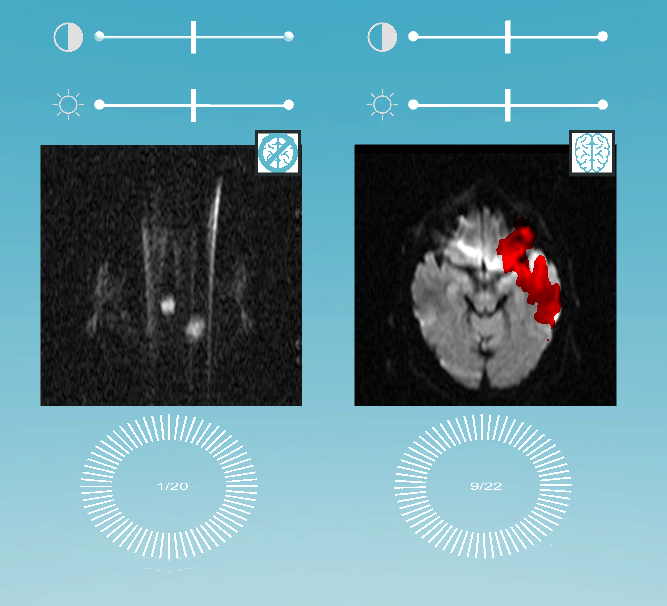
\includegraphics[width=0.5\linewidth]{images/mARt2d.png}
	\caption{Die zweidimensionale Darstellung von zwei MRT-Datensätzen, deren Manipulation nicht gleichgeschaltet ist. Über die oberen Schieberegler können Kontrast und Helligkeit beeinflusst werden. durch das Icon in der rechten Ecke kann der markierte Bereich ein- und ausgeblendet werden. Das Rad ermöglicht das Scrollen durch die Bildschichten. Die aktuelle Schicht wird in dessen Mitte angezeigt. }
	\label{img:mARt2d}
\end{figure}


\begin{figure}
	\centering
	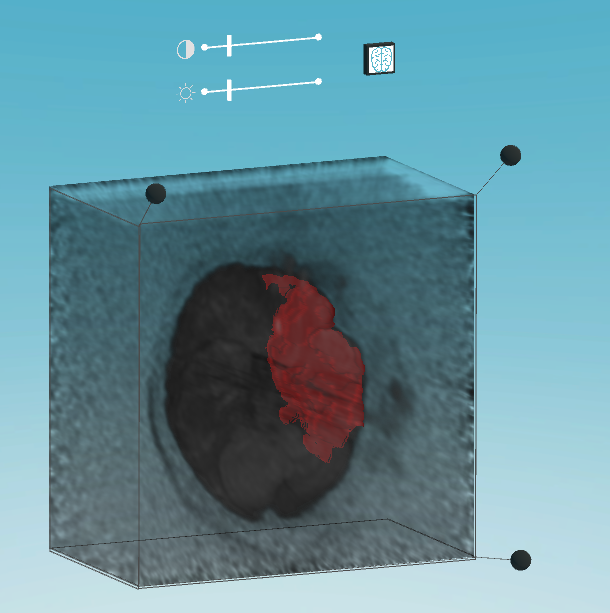
\includegraphics[width=0.5\linewidth]{images/mARt3d.png}
	\caption{Die 3D-Darstellung eines MRT-Datensatzes mit angezeigter Maske. Die oberen Schieberegler kontrollieren Intentsität und Schwellenwert des Renderings. Auch hier wird der markierte Bereich durch ein Icon ein- und ausgeblendet. Jede Ebene kann durch einen Anfassungspunkt verschoben werden.}
	\label{img:mARt3d}
\end{figure}


Der Use Case \textbf{U04} erfordert es weiterhin, dass man Bilder im direkten Vergleich nebeneinander betrachten kann. Dies gilt sowohl für die zwei- als auch dreidimensionale Darstellung der Daten. Die UseCases \textbf{U05} und \textbf{U06} erfordern außerdem eine Möglichkeit für den Nutzen aus den vorhandenen Daten einzelne auszuwählen, die angezeigt werden sollen, sowie die Daten jeweils gleichzeitig oder einzeln zu manipulieren. 
Die Auswahl der Datensätze, sowie die Wahl ob diese synchron manipuliert werden sollen oder nicht, sind beide nicht Teil der direkten Manipulation des Bildes. Sie müssen deshalb nicht in dessen unmittelbaren Umfeld stehen und der Nutzer kann während dessen Bedienung auch auf diese den Fokus setzen.
 
Die Bedienung der entsprechenden Interaktionselemente sollte trotzdem intuitiv und schnell umzusetzen sein. Da die Option der Synchronizität abhängig ist von der Tatsache, ob ein oder mehrere Datensätze angezeigt werden, stehen die beiden Aktionen in Verbindung zu einander und werden deshalb in einem Menü vereint, das für beide Darstellungen verwendet wird. Dieses wird an der linken Hand des Nutzers verankert. Auf diese Weise kann es immer schnell erreicht werden und wird nicht unbeabsichtigt aus den Augen verloren. Gleichzeitig fördert es die Immersion der Anwendung, da der Nutzer quasi Teil von ihr wird. Ein Effekt, der in einer Bildschirmanwendung nicht umsetzbar wäre. 

Damit das Menü nicht wären der Verarbeitung der Bilder stört, wird es nur dann eingeblendet, wenn der Nutzer seine Handfläche Richtung Kamera dreht und diese somit ansieht. Motion Leap bietet bereits Beispiel Code, der dies umsetzt. ?
Eine besondere Herausforderung bei der Konzeption des Menüs ist es, dieses möglichst einfach und platzsparend zu halten. Das Erfassungsfeld der Motion Leap Kamera, in dem die Hände erkannt werden ist beschränkt. Deshalb kann es bei einer Interaktionsfläche die viel Raum davon einnimmt dazu kommen, dass der Nutzer versehentlich Knöpfe betätigt. 
Um den Umfang des Menüs in benutzbaren Dimensionen zu halten wurde es auf drei Knöpfe reduziert. 
Die Liste der verfügbaren Datensätze kann darin allerdings nicht untergebracht werden. Deshalb kann sie bei Bedarf über einen der Knöpfe ausgeklappt werden. 
Indem der Nutzer einen Datensatz auswählt, wird dieser auf der Bildfläche angezeigt. Die Auswahl ist auf zwei Datensätze beschränkt. Zu viele gleichzeitig dargestellte Bilder würden unübersichtlich wirken und die Motivation hinter dem Use Case ist der direkte Vergleich zweier Bilder. Außerdem stellen mehr Bilder auch mehr Möglichkeiten dar diese in verschiedenen Kombinationen zu manipulieren. Dies hätte die Anwendung unnötig verkompliziert. 
Stattdessen wird die Synchronisierung der Manipulation über einen weiteren Knopf im Handmenü gesteuert. Dieser ist nur aktiv, wenn tatsächlich zwei Bilder angezeigt werden. Dann funktioniert er als Schalter. Indem der Nutzer in betätigt wird jeweils nur eine Benutzeroberfläche neben beiden Bildern angezeigt oder sie wird dupliziert und für jede Darstellung eingeblendet. 
 
Schließlich kann der Nutzer durch das Handmenü auch zwischen der zwei- und dreidimensionalen Darstellung wechseln, wie es in \textbf{U09} beschrieben ist. Auf dem dafür zuständigen Button wird jeweils das Szenario angezeigt, in das gewechselt wird.
Laut \textbf{U10} sollen beim Wechsel die Manipulationen und Einstellungen möglichst erhalten bleiben. D.h. wenn in 2D zwei Datensets angezeigt werden, eines mit und eines ohne Maske, sollte das nach dem Wechsel zu 3D ebenfalls so sein. 

//TODO: Ist das so?

In Abbildung \ref{img:handUI} ist das ausgeklappte Menü, an der linken Hand dargestellt.

\begin{figure}
	\centering
	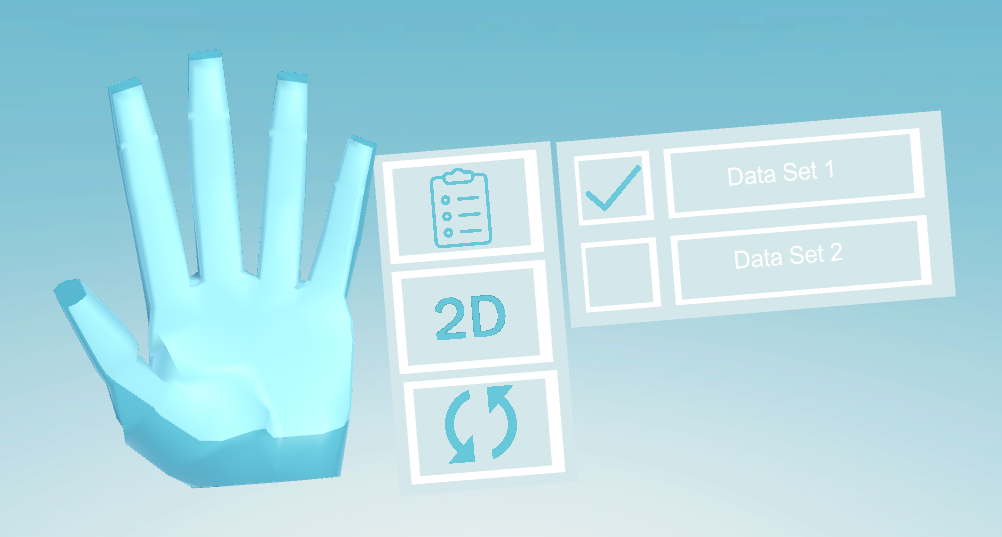
\includegraphics[width=0.7\linewidth]{images/handUI.png}
	\caption{Das ausklappbare Handmenü, das erscheint, wenn der Nutzer seine Handfläche zur Kamera dreht. Über die Knöpfe kann der Nutzer die angezeigten Datensätze auswählen (oberen und Liste), zwischen 2D- und 3D-Darstellung wechseln (mitte) und die angezeigten Datensätze gleichschalten (unten). }
	\label{img:handUI}
\end{figure}

//TODO:
bezug zu interaktion in grundlagen

Die Darstellung der MRT-Daten soll, wie in Anforderung \textbf{U16} beschrieben im Raum platzierbar sein und nach \textbf{U17} ihre Position dort behalten, sodass der Nutzer um sie herum gehen und von allen Seiten betrachten kann, oder an einem bestimmten Standpunkt verankern kann. Dies wäre vor allem in einem Multi-Nutzer-Szenario nützlich, in dem mehrere Nutzer gleichzeitig die Daten betrachten.
Die Hololens bietet diese Funktionalität in Form von Spatial oder World Anchors. Das Gerät besitzt einen internen Speicher für Anker, die von einer Anwendung angelegt werden, den sogenannten Anchor Store. Durch interne Prozesse bestimmt die Hololens in welchem Raum sie sich gerade befindet. Wird ein World Anchor in diesem Raum abgelegt, wird dessen Standort im Anchor Store gespeichert und behält somit immer seine Position im Raum, auch wenn der Nutzer sich bewegt und über mehrere Sitzungen hinweg. Nachdem ein World Anchor beim Start der Anwendung geladen wird, kann er an ein Objekt, wie ein 3D-Modell anhängt werden, sodass das Objekt an der Position des Ankers dargestellt wird. 

Der Anchor Store ist allerdings, wie beschrieben nur auf der Hololens verfügbar. Wie im Kapitel \ref{implementierung} erläutert wird, wird die Anwendung im Rahmen dieser Arbeit aber nur auf der Hololens abgespielt, aber nicht deployed. Dementsprechend ist ein Zugriff auf den Anchor Store nicht möglich. Dasselbe gilt für eine Verwendung der Anwendung in einem VR-System.

Als Alternative dazu könnten die Daten mit Hilfe eines Markers in den Raum projiziert werden, wie es im Kapitel \ref{grundlagen} beschreiben wurde. Unity bietet hierfür das Vuforia-Plugin, welches genau das umsetzt. Hierzu können Marker definiert werden, die das Programm erkennt und die diesen zugeordneten GameObjects anzeigt. 
Vuforia ist für AR-Anwendungen gedacht, und funktioniert durch eine Kamera, die den Marker erkennt. Deshalb könnte die Funktion von einer HTC Vive nicht genutzt werden, von einer HTC Vive Pro jedoch schon, da diese über einen Mixed Reality Modus verfügt. Auch Hololens-Anwendungen können Vuforia nutzen. 

Im zeitlichen Rahmen der Arbeit konnte dieses Funktionalität allerdings nicht mehr umgesetzt werden.

//TODO 
Bezug zu Anforderungen

\subsection{Interaktion AR}

Die Interaktionen bleiben in der AR- und VR-Version der Anwendung gleich, da für beide die Leap Motion zur Steuerung verwendet wird.
Im Gegensatz zum Einsatz in VR sind allerdings die realen Hände des Nutzers für diesen sichtbar, während er die Anwendung in AR bedient. Da durch die Leap Motion die Hände zusätzlich virtuell simuliert werden, sieht der Nutzer vier Hände, was zuerst verwirrend wirken kann. 
Die Leap-Controller-Hände für den Nutzer unsichtbar zu machen, wäre zaw möglich, ist allerdings nicht die beste Vorgehensweise. Obwohl die Leap Motion die Hände und Handbewegungen sehr zuverlässig nachempfindet, verhalten die virtuellen Hände sich nicht ganz deckungsgleich zu den realen. Dies hängt auch damit zusammen, dass die Leap Motion Kamera sich ein Stück vor oder über den Augen des Nutzers befindet, da sie am HMD befestigt ist. Dieses Problem wird auch in Abschnitt \ref{kombination} beschrieben.
Die Abweichungen der Simulation sind in einer VR-Anwendung deutlich weniger auffällig. Durch die Immersion der virtuellen Welt und dem Fehlen eines direkten Vergleichs mit der realen, entsteht beim Nutzer die Illusion, dass die virtuellen Hände sich genau dort befinden, wo er seine echten Hände vermutet.

In AR entfällt diese Illusion. Da die beiden Hände Paare aber nicht deckungsgleich sind, kann es dazu kommen, dass ein virtueller Finger einen Knopf trifft, während es ein realer nicht tut oder umgekehrt. Wenn der Nutzer die virtuelle Hand nicht sieht, würde dies den Eindruck von fehlerhaftem Verhalten hervorrufen. 
Aus diesem Grund werden die Leap-Controller-Hände auch in der AR-Anwendung angezeigt. Allerdings werden sie leicht transparent dargestellt, um dem Nutzer zu erlauben auch die dahinter liegende Umgebung wahrzunehmen. 

TODO: 
Bild AR Hände


\section{Unterstützung von Dateiformaten} 

In den im Kapitel \ref{anforderung} beschriebenen Anforderungen ist durch \textbf{U19} und \textbf{U20} beschrieben, dass mARt gängige Dateiformate zur Speicherung von medizinischen Bilddaten, insbesondere NIfTI und DICOM unterstützt. Beide Formate wurden im Kapitel \ref{grundlagen} beschrieben. 
Unity unterstützt diese Formate nicht. Um die MRT-Bilder also zu verarbeiten und darstellen zu können, muss eine Parser oder Converter in das Programm eingebunden werden. 
Der Nutzer könnte dann über eine Schnittstelle die Daten direkt in die Anwendung laden, wo sie umgewandelt und angezeigt würden. 

In einer realen Arbeitsumgebung ist diese Funktionalität mehr als sinnvoll. Wie allerdings in \ref{anforderung} beschrieben, soll es sich bei mARt in erster Linie um einen Prototyp handeln.
Der Fokus soll dabei auf der Darstellung der Daten und der Interaktion mit ihnen liegen. Da der zur Entwicklung und zum Testen zur Verfügung stehende Datensatz gering ist, ist die Nützlichkeit in diesem Szenario nicht gegeben. Der benötigte Zeitaufwand zur Implementierung wird somit nicht durch einen Mehrwert gerechtfertigt.
Weiterhin kann so die Komplexität und der Umfang der Anwendung gering gehalten werden, was es dem Nutzer erlaubt sich auf die Kernfunktionen zu konzentrieren. 

Durch den eingeschränkten verfügbaren Datensatz, konnte auch \textbf{U18}, nicht umgesetzt werden, da es keine Scans verschiedener Frequenzen des selben Datensatzes gab.

Trotzdem können mehrere Datensätze in mARt dargestellt werden. Diese werden durch Verwendung der externen Bildsoftware ImageJ manuell in PNG-Dateien umgewandelt und in die Anwendung integriert, bevor diese gebaut wird. 
Obwohl dieser manuelle Vorgang umständlich ist, ist er für dden Zweck der Anwendung und den Umfang dieser Arbeit ausreichend.
